\chapter{Implementation}

This chapter details the implementation of Snapstore. That includes relevant implementation decisions, the current status of Snapstore, and important algorithms. 

Snapstore was built to be cross-platform using Electron\footnote{http://electron.atom.io/}. We used web sockets\footnote{www.socket.io} for networking. Once a client is connected over a socket, Snapstore can be constantly pulling in and pushing out new snapshots that come in from that user and from other users. Sockets provide the additional benefit of allowing us to group users. We used this functonality to make ``rooms'' of users that have read and write access to a specific branch. Pushing changes on that branch out to those users is simple with sockets.

\section{Data Structures}

\subsection{Client}

Each local repository on the client has its own mongo database. Each database has a collection of snapshots, branches, groups, tags, and events. It also has one snapstore document and a binary large object (blob) collection. A data model representing each data structure and its attributes can be found in figure 4-1.

\begin{figure}
\includegraphics[max width= \linewidth]{DataModel}
\caption{Snapstore client data model.}
\label{arm:fig1}
\end{figure}

When a file is saved, the resulting snapshot must first decide what kind of snapshot it is. Whether it is a create, update, rename, delete, merge, or conflict snapshot dictates how it will populate its data fields. A create snapshot, for example, has no parent snapshot. When any snapshot is created, it is added to the collection of snapshots, and the branch updates its list of head snapshots to include this new snapshot, while removing its parent.

If two snapshots have the same content, they point to the same blob data in the blob collection to save space. This blob collection holds hashes of the content along with the binary content.

When a new branch is created, it is added to the database with only a name. If, however, it was cloned from another branch, the cloned branch will point to all head snapshots, groups, and tags from the original branch. When switching to a branch, the heads snapshots for the target branch are read and applied to the Snapstore folder. To read the history of a file, the head snapshot of the file is located, and the rest is found by searching backwards through the snapshot graph.

The event collection stores all of the unconfirmed snapshots, groups, and tag events on the client. As these events are confirmed, they are erased from the collection.

\subsection{Upstream}

On the upstream server, the snapshot, branch, group, tag, and content data structures are the exact same as those on the client. They are kept consistent with each local repository when a socket connection is open. A model of the data structures on the upstream is show in figure 4-2.

\begin{figure}
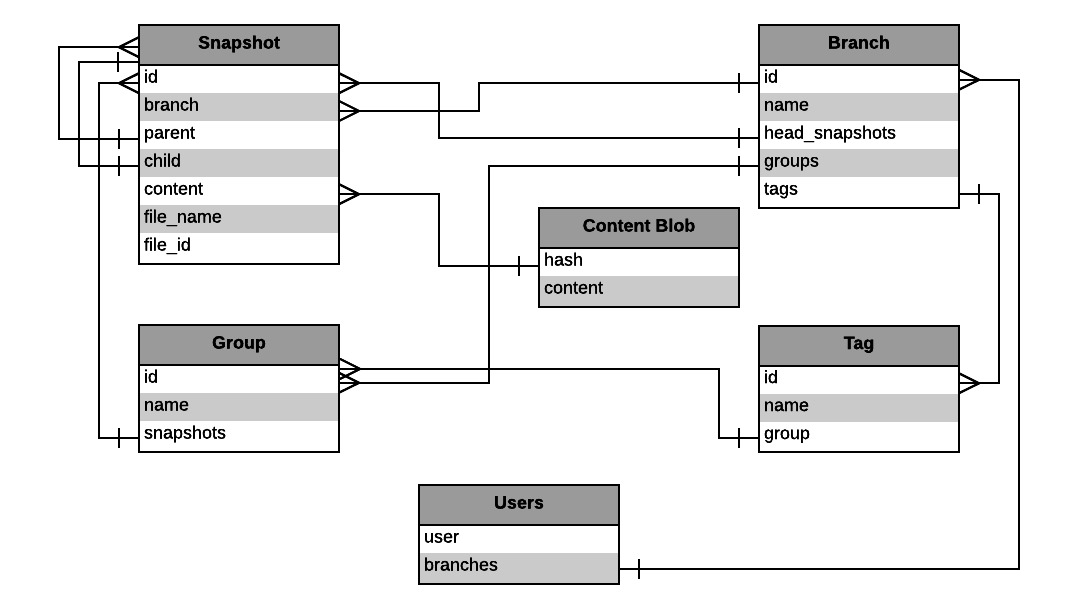
\includegraphics[max width= \linewidth]{DataModelServer}
\caption{Snapstore server data model.}
\label{arm:fig1}
\end{figure}

The user model on the server is a mapping of users to branches to which they have access. It uses this mapping to add users to appropriate socket rooms when they connect to the Snapstore server. Once users are in those rooms, they can be updated with changes to that branch.

\section{User Interface}

**Pictures will go in here when the UI is done.**

\section{Keeping Data in Sync}

\subsection{Shared Branches}

For Snapstore, we wanted users to be able to work on a shared branch. As described in section 2.2.3, a shared branch is a line of development where a change from one user is propagated to all other users on that line as soon as a network connection is available. If there are multiple connected users on a shared branch, a change made by one of them should result in changes to the filesystems of all other users, so as to keep all local working directories consistent.

We have opted to use a last-write-wins appraoch when dealing with conflicts on a shared branch because it is an easier paradigm for non-technical users to understand compared with merging. Plus, with the potential amount of conflicts on a shared branch, the number of merges would be very high. Because of this, merging is only done between branches on the local repository.

This approach can result in a snapshot being very far removed from their original parent. For example, say Alice and Bob share a branch with a single snapshot. Alice goes offline and makes one snapshot of her own. Bob, still online, makes 10 snapshots that are immediately confirmed by the server. When Alice returns to the network, her snapshot would be placed after Bob's 10 confirmed snapshots, far from its original parent.

Despite this, we believe this approach is appropriate for two reasons. First, in the current highly connected environment of today's computing, making that many offline edits is typically done by choice. Second, if offline edits are indeed an issue, Snapstore allows users to create a separate branch for highly disconnected development. 

\subsection{Network Issues}

The workflow described in section 4.3.1 can be difficult to maintain. Multiple users can be making multiple edits at the same time, increasing concurrency issues. If two snapshots are made at the same time, there needs to be a way to resolve the snapshot graph and propagate it to all collaborators on a branch. Network concerns and partitions increase the difficulty and uncertainty of this problem. 

Imagine a user goes offline and makes multiple snapshots and groups, all while their shared file is being written to by other, online users. Snapstore should be able to handle their reintroduction to the network without destroying the branch history.

We take the approach that any data that reaches the upstream server and is confirmed should be regarded as fact; they should not be undone. With this invariant, we designed a protocol algorithm for this process, called Distributed Event Sychronization Queue (DESQ).

\subsection{DESQ} 

\begin{center}
\begin{algorithm}
\caption{DESQ}\label{euclid}
\begin{algorithmic}[1]
\Procedure{Client-DESQ}{}
\State $\textit{events} \gets \text{collection of }\textit{Events}$
\State $\textit{socket} \gets \text{server socket connection}$
\While {\emph{events} not empty}
\State $socket\text{.send(}events(0)\text{)}$
\EndWhile
\Loop{ on \emph{socket}.reponse(\emph{response, message})}:
\State Save \emph{response}
\If {$message == \text{"Confirmed" or "Duplicate"}$}
\State \emph{events}.remove(\emph{response})
\EndIf
\EndLoop
\EndProcedure
\end{algorithmic}
%%%%%%%%%%%%%%%%%%%
\begin{algorithmic}[1]
\Procedure{Server-DESQ}{}
\State $\textit{db} \gets \text{MongoDB}$
\State $\textit{socket} \gets \text{client socket connection}$
\Loop{ on \emph{socket}.receive(\emph{event})}:
\If {$\textit{event} \text{.data.id in } \textit{db}$}
\State return $\text{"Duplicate Event"}$.
\EndIf
\If {$\textit{event}\text{.type } != \text{snapshot}$}
\State $event\text{.confirmed} \gets \text{True}$
\State $socket\text{.send(}event, \text{"Confirmed")}$
\State $socket\text{.room.send(}event, \text{"New Event")}$
\Else
\If {$event\text{.data.parent is head snapshot}$}
\State $event\text{.confirmed} \gets \text{True}$
\State $socket\text{.send(}event, \text{"Confirmed")}$
\State $socket\text{.room.send(}event, \text{"New Event")}$
\Else
\State $conflictSnapshots \gets \text{All snapshots between }event\text{ and }event\text{.parent}$
\State $socket\text{.send(}conflictSnapshots\text{,"Reject Event")}$
\EndIf
\EndIf
\EndLoop
\EndProcedure
\end{algorithmic}
\end{algorithm}
\end{center}

Each client will have their own ordering of events. These events are any database operation, and they are stored in a client queue until they are confirmed by the server. The DESQ algorithm seeks to reach eventual consistency between these client queues so that every client has the same data.

It is also important to maintain the ordering of events created by a single user. If a user creates a snapshot and then creates a group with that snapshot it in, it is necessary to send those two events in order to the server. Otherwise, the server will try to create a group containing a snapshot that doesn't exist.

When a new action in the database is triggered, that event data is saved to the client event queue. This queue, by itself, is a guaranteed in-order sequence of all database actions by the client. Each event in the queue is related to its parent and its child by a pointer, and these pointers are used to detect inconsistencies. If the client is working by themselves, in their own branch, this queue will simply be mirrored by the server when the network in connected. If the client is working with another client on the same branch, there may be concurrent events being sent to the server, resulting in ordering issues.

This algorithm tries to push these events to the server repository. In Git terms, if there is a conflict, the branch rebases and tries to push that event again. This continues until all events are successfully pushed. The rebasing keeps the snapshot graph and the workflow for the branch linear. However, while Git creates new commits during a rebase, Snapstore uses existing snapshots in the resulting snapshot graph.

DESQ begins when an inconsistency is detected in the system. This can happen in two ways. First, if there is an event in the client's event queue, the algorithm will try to get that event confirmed by the server and shared with all appropriate users. Second, if a client connects to the server and detects that changes have been made, it will pull in those changes. Once the algorithm begins, it will not stop until the inconsistencies are resovled. 

Note that this protocol can proceed only when network connections between the server and client are open. If they are closed, the events are queued in the client until the network is available. Then, they are processed in the same way.

\subsubsection{Confirmed Events}

Events are always confirmed unless they are a snapshot event whose parent is not a head snapshot on the server. Lines 9 and 14 of the pseudo-code for Server-DESQ show a particular event being confirmed by the server. On the client machine, the event is registered as confirmed and removed from the event queue.

\subsubsection{Receiving Events From the Server}

When a client sends an event to the server and it is confirmed, the event must be propagated to all other collaborators. The server will find all clients that have access to that event's branch and send it to them. Because this is a confirmed event coming from the server, the other clients can apply this event to their local repository.

This process can be happening while a client is offline. As stated above, when the client returns to the network, it will be pushed all of these events from the server so that it can update its queue. 

\subsubsection{Rejected Snapshots}

DESQ's last-write-wins approach only applies to snapshots because they are the only type of event that can cause a conflict, due to their inclusion in a snapshot graph. The server, for each snapshot event it receives, will always verify whether it has seen a different snapshot event from another client in the meantime.

If the server has seen other snapshots, making the server's history inconsistent with the client's history, it rejects the client's snapshot event. The rejected snapshot then goes back to the client, along with the snapshot(s) that caused the rejection. The snapshot(s) that caused the rejection are found by traversing the server's snapshot graph from the rejected snapshot's parent to the head. These additional snapshots are inserted at the end of the client's snapshot graph, but before the rejected snapshot. The rejected snapshot is sent to the server again for confirmation, restarting the algorithm. 

Because the rejected snapshot is kept at the front of the event queue to be sent to the server, this process can continue without disrupting the inherent correct ordering of events for a single client. So, if a client has made multiple offline events, only the first of those could trigger the rejection.

This protocol allows the system to handle consecutive rejections. This can occur when other clients are sending snapshot events to the server while another client's event is being rejected.

\subsubsection{Duplicate Events}

In the case of network outages, it could be the case that the client goes down before the server can respond that it has received an event. In this case, when the client comes back online, it will retry to send that event. Because the ID of that event's data already exists on the server, it will simply respond that it has already received the event. This will allow the client to confirm the event.